\section{Experimentación}

En este apartado se realiza una explicación en profundidad de las pruebas que se han realizado
para validar y verificar la implementación descrita en apartados anteriores. Esta sección incluye
la explicación en detalle de todo el diseño experimental llevado a cabo, incluyendo las técnicas
a comparar, la descripción del \textit{dataset} utilizado para la experimentación, el
procedimiento seguido para realizar el entrenamiento y prueba de los modelos, incluyendo el
\textit{key-fold cross-validation}, la descripción del cálculo de las distintas métricas de
evaluación y, finalmente, los resultados obtenidos y su correspondiente análisis. Además, en esta
última sección, se dará respuesta a las preguntas de investigación planteadas en la Sección
\ref{sec:research_questions}, lo que constituye el objetivo principal de este estudio.

\subsection{Diseño experimental}
\noindent En esta sección se describe el diseño experimental llevado a cabo para la validación
de la implementación propuesta.

\subsubsection{Técnicas a comparar.}
En este estudio, se propone comparar tres técnicas de predicción diferentes. Por un lado, la
propuesta en \textit{SmartBuildSkip} \cite{2} que usa bosques aleatorios en su algoritmo de
predicción y, por otro lado, las dos técnicas propuestas en este estudio, JAES24. A continuación,
se describen las tres técnicas a comparar:

\begin{itemize}
    \item \textbf{SBS-Within}: técnica propuesta en \textit{SmartBuildSkip} que utiliza bosques
    aleatorios en su algoritmo de \textit{Machine Learning} para la predicción. Esta técnica
    tiene dos fases principales: una en la que el algoritmo predice de forma automática que
    la \textit{build} fallará, por encontrarse en una secuencia de \textit{build failures}, y
    otra en la que utiliza predicción mediante \textit{Machine Learning}.\\

    \item \textbf{JAES24-Within}: técnica propuesta en este estudio que utiliza como modelo de
    ML áboles de decisión. El algoritmo de predicción se basa en la implementación propuesta de
    \textit{SmartBuildSkip}, pero modificando el conjunto de \textit{features} empleado: TF, NC,
    FC, LC, LA, LR, LT, WD y DH, el cual captura eventos temporales al realizar las \textit{builds}
    y desgrana los cambios realizados en la misma. Además, en este algoritmo se realiza la
    acumulación de \textit{features}, lo cual permite acumular cambios para la predicción cuando
    una \textit{build} es saltada por el algoritmo.\\
    
    \item \textbf{JAES24-Without}: técnica propuesta en este estudio que utiliza como modelo de
    ML árboles de decisión. Este modelo emplea el mismo conjunto de \textit{features} descrito en
    el punto anterior, sin embargo, no utiliza como base la implementación realizada
    \textit{SmartBuildSkip}, por lo que no se realiza acumulación de valores en las \textit{features}
    cuando una \textit{build} es saltada por el algoritmo, ni tampoco tiene dos fases de predicción.
    En este caso, simplemente se van realizando predicciones de forma individual para cada
    \textit{build}.
\end{itemize}

Dependiendo del contexto sobre el que se realicen las predicciones, puede ser más adecuado
utilizar una técnica u otra. Por ejemplo, si el proyecto sobre el que realizamos predicciones
suele tener muchos \textit{build failures} de forma consecutiva, será más beneficioso utilizar
las técnicas \textit{SBS-Within} o \textit{JAES24-Within}, ya que estas tienen una fase
en la predicción especialmente diseñada para detectar secuencias de \textit{build failures}. Por
otro lado, si el proyecto tiene \textit{build failures} producidos más aleatoriamente a lo largo
del proyecto, será más beneficioso utilizar la técnica \textit{JAES24-Without}, ya que esta no 
tiene en cuenta secuencias de \textit{build failures} en su algoritmo de predicción.\\

Realizar una comparación entre estas tres técnicas nos da una visión más amplia de los
resultados obtenidos en este estudio, permitiéndonos identificar cual de ellas es más adecuada en
términos de precisión, eficiencia o adaptabilidad a las características del problema. El hecho
de considerar varias técnicas mejora la validez interna del estudio, ya que se descarta que los
resultados sean atribuibles a una sola metodología.

\subsubsection{Descripción del \textit{dataset}.}
Para realizar la experimentación, se han utilizado $20$ proyectos de código abierto disponibles
de forma pública en \textit{GitHub}. Todos los proyectos están basados en \textit{Java} y
han sido seleccionados de forma manual. Con el objetivo de tener una experimentación diversa,
se han tenido en cuenta dos escenarios posibles:

\begin{enumerate}
    \item \textbf{Escenario 1}: engloba a todos aquellos proyectos donde la  CI falla con muy
    poca frecuencia. En nuestra solución, se ha considerado a todos estos proyectos como
    ``proyectos difíciles'', y serán todos aquellos en los que la proporción de \textit{build
    failures} es inferior al $10\%$ con respecto a las \textit{builds} exitosas.\\

    \item \textbf{Escenario 2}: engloba a todos aquellos proyectos donde la CI falla con
    una frecuencia ``normal''. Consideramos como ``proyectos normales'' a todos aquellos en los
    que el porcentaje de \textit{build failures} se encuentra comprendido entre el $10\%$ y el
    $25\%$ con respecto a las \textit{builds} exitosas.
\end{enumerate}

Al incluir tanto proyectos difíciles como normales, se pretende obtener una visión más amplia
de la efectividad de nuestro algoritmo en diferentes condiciones y escenarios. Este enfoque
es beneficioso por varias razones:

\begin{itemize}
    \item \textbf{Evaluación en escenarios específicos}: separar ambos escenarios nos permite
    analizar el comportamiento del modelo en cada tipo de proyecto de forma más precisa.\\

    \item \textbf{Fortalezas y debilidades}: al evaluar cada conjunto de proyectos individualmente,
    podemos identificar fortalezas y debilidades del modelo en cada escenario.\\

    \item \textbf{Adaptabilidad del modelo}: al evaluar el modelo en diferentes escenarios, podemos
    observar si el modelo es capaz de adaptarse bien a ambos tipos de proyectos, o si realmente
    necesita un enfoque diferente para cada uno de ellos.
\end{itemize}

Se ha decidido catalogarlos como ``proyectos difíciles'' y ``proyectos normales'' según la
capacidad que tendrá el algoritmo de aprender de los \textit{build failures} en cada tipo de 
proyecto. En los proyectos difíciles, donde se espera que la proporción de \textit{build
failures} sea mucho menor a la de \textit{builds} exitosas, el algoritmo tendrá que aprender
de un número mucho menor de ejemplos de fallos, haciéndole la tarea de aprendizaje más difícil.
Por otro lado, en los proyectos normales, donde la proporción de \textit{build failures} es
más alta, el algoritmo tendrá más ejemplos de \textit{build failures} sobre los que aprender,
esperando que la capacidad de aprendizaje sea mayor.\\

Como hemos mencionado anteriormente, se han seleccionado $20$ proyectos de código abierto
disponibles en \textit{GitHub}. Cada uno de ellos ha sido seleccionado de forma manual, y se
ha intentado que el número de \textit{builds} sea lo más similar posible entre ellos. A
continuación, se muestran dos gráficos que describen la proporción de \textit{build failures}
en cada uno de los proyectos seleccionados, tanto para proyectos difíciles como para proyectos
normales.\\

\begin{figure}[H]
    \centering
    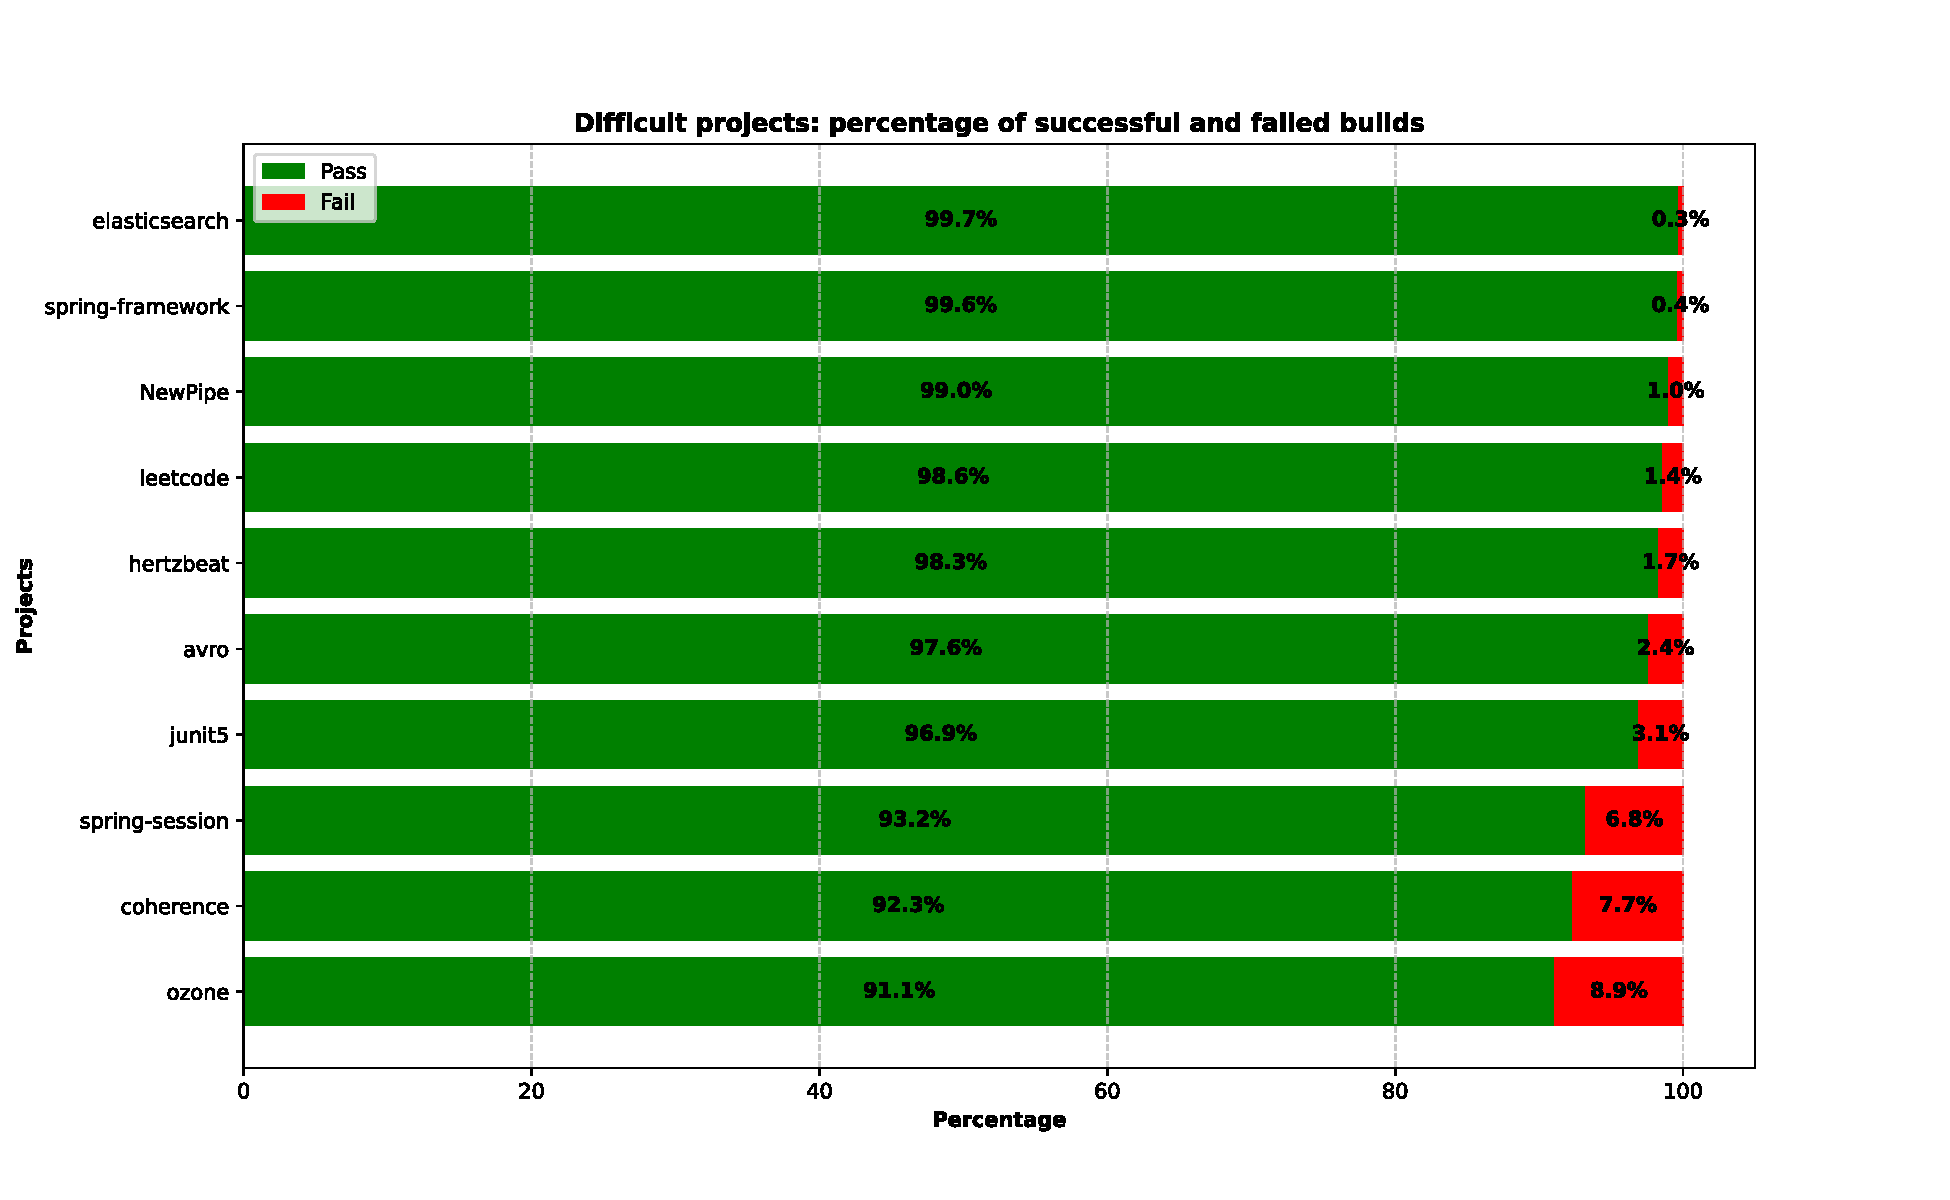
\includegraphics[width=0.85\textwidth]{images/Failures_difficult_projects.pdf}
    \caption{Proporción de \textit{build failures} en proyectos difíciles}
    \label{fig:failures_difficult_projects}
\end{figure}

\begin{figure}[H]
    \centering
    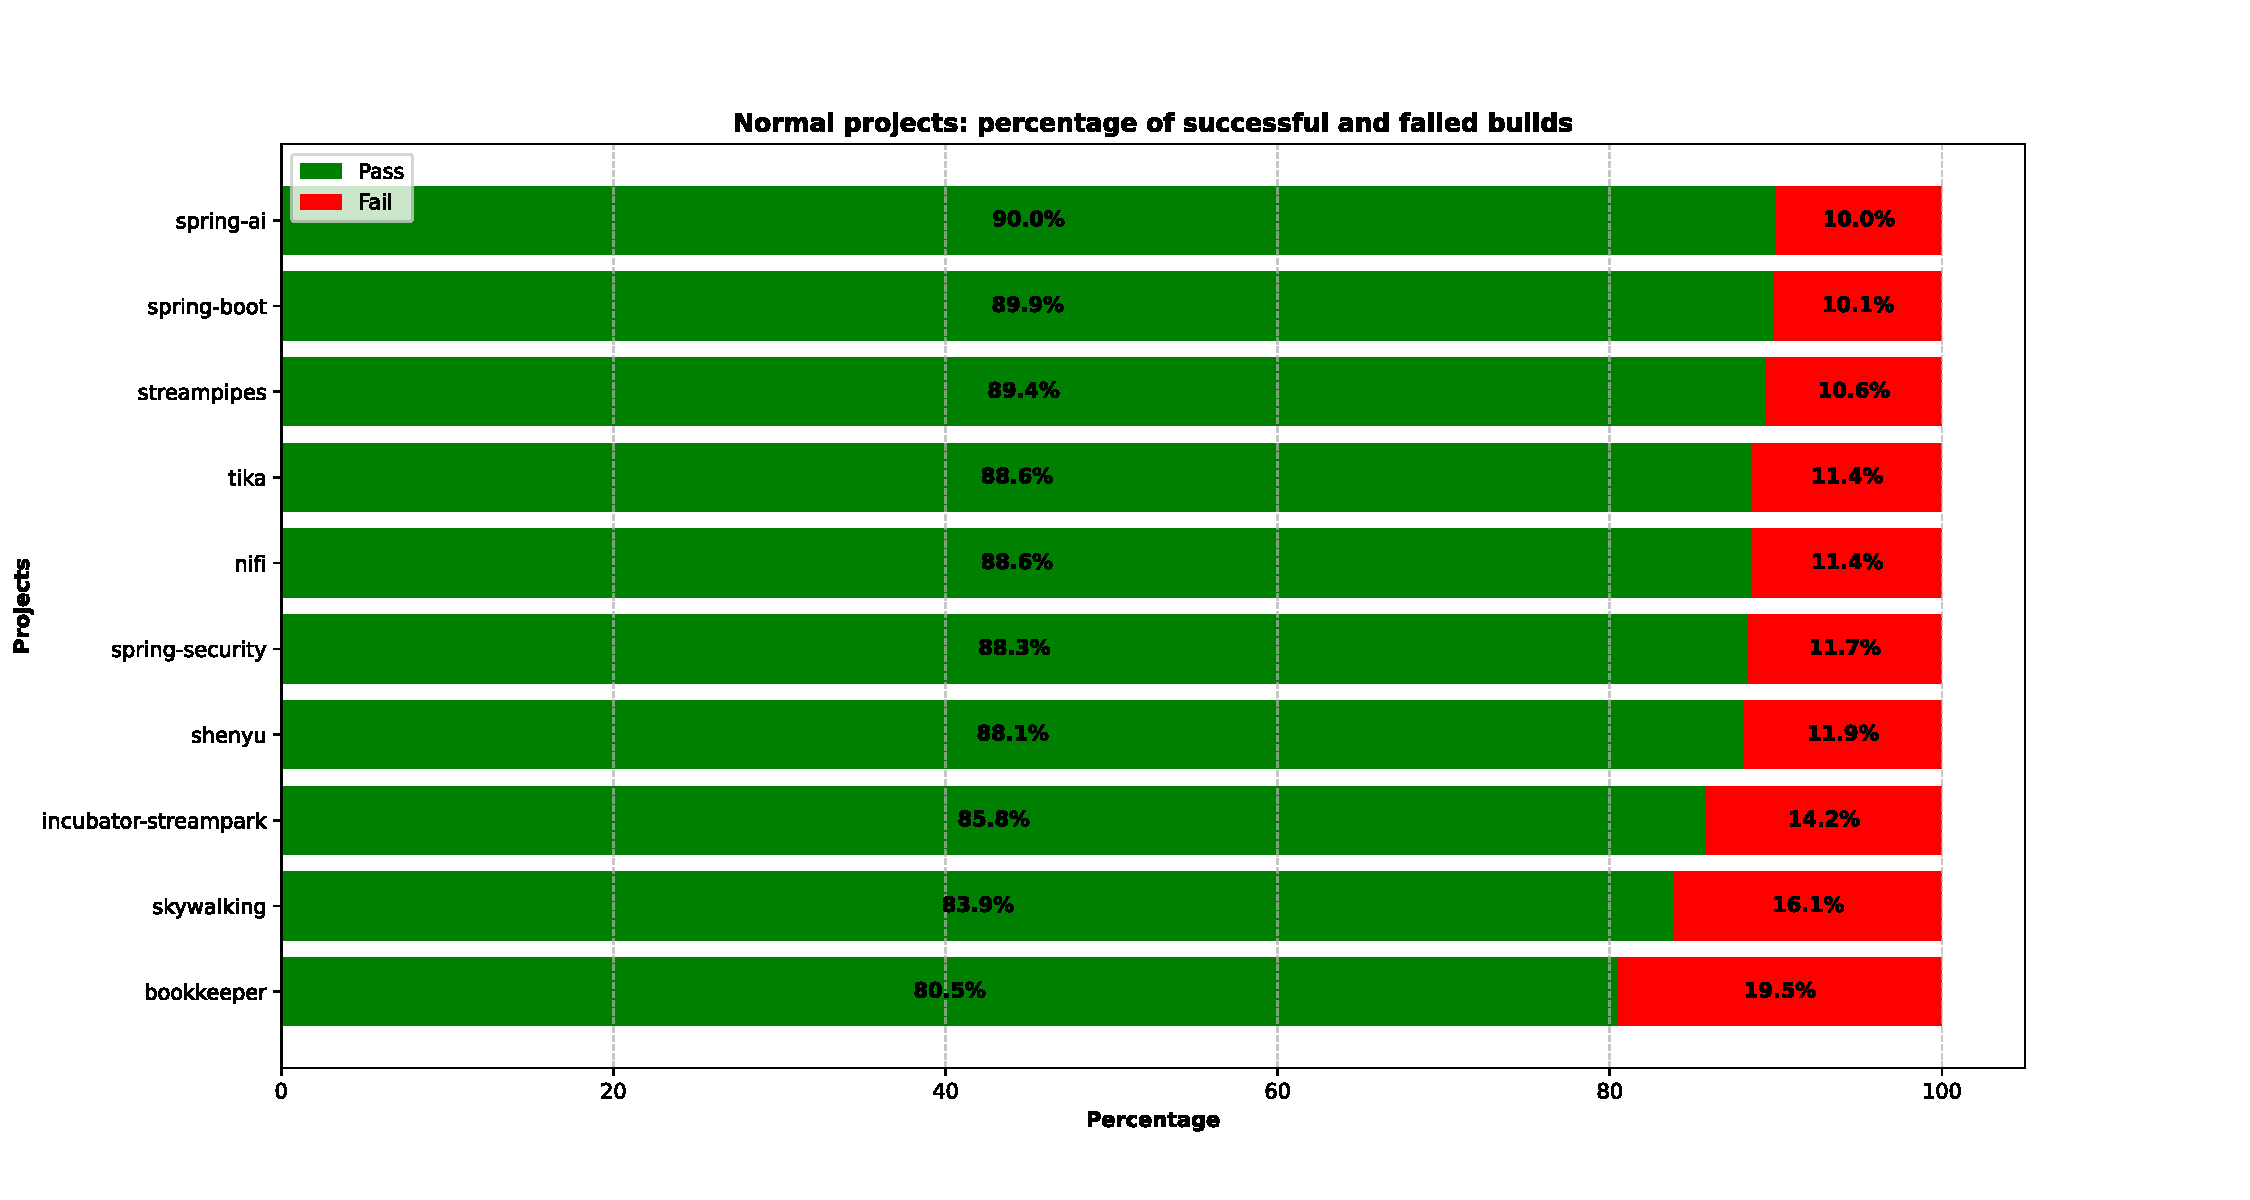
\includegraphics[width=0.85\textwidth]{images/Failures_normal_projects.pdf}
    \caption{Proporción de \textit{build failures} en proyectos normales}
    \label{fig:failures_normal_projects}
\end{figure}

Como vemos, en los proyectos difíciles la proporción de \textit{build failures} es inferior al
$10\%$, mientras que en los proyectos normales se encuentra entre el $10\%$ y el $25\%$. En
ambos casos, se ha intentado que el número de \textit{builds} sea lo más similar posible entre
los proyectos seleccionados.\\

\subsubsection{Procedimiento para el entrenamiento, prueba  y validación cruzada}
La evaluación de los modelos de clasificación busca medir y analizar el desempeño de los mismos
en la tarea de clasificación. Esta evaluación permite determinar la capacidad del modelo para
predecir o clasificar correctamente nuevas instancias no observadas previamente, utilizando un
conjunto de datos de prueba.\\

\noindent Para cada uno de los $20$ proyectos seleccionados, se ha realizado lo siguiente:


\begin{enumerate}
    \item \textbf{Conjunto de entrenamiento y prueba}: se ha dividido el subconjunto de
    \textit{builds} en dos subconjuntos, uno de entrenamiento y otro de prueba. El porcentaje
    de entrenamiento y prueba se ha fijado en $80\%$ y $20\%$ respectivamente. Se ha tenido
    especial cuidado en seleccionar el $80\%$ de las \textit{builds} más antiguas para el
    subconjunto de entrenamiento y, el $20\%$ de las \textit{builds} más recientes para el
    subconjunto de prueba. Esto es así por la dependencia temporal que existe en este tipo de
    problemas, donde no tiene sentido realizar predicciones basándonos en información futura.
    Además, para realizar este entrenamiento y prueba, se ha escogido el umbral de decisión
    por defecto, con valor $0.5$.\\

    \item \textbf{Key-fold cross-validation}: se ha utilizado la técnica de validación cruzada
    \textit{key-fold cross-validation} para evaluar el rendimiento de los modelos de clasificación
    propuestos. Para cada proyecto, se han seleccionado sus \textit{builds} y se han creado $11$
    subconjuntos a partes iguales. A continuación, se ha realizado la validación cruzada de
    la siguiente forma: se han ido seleccionando los \textit{folds} de forma acumulativa para
    realizar el entrenamiento, mientras que con el \textit{fold} siguiente se ha realizado la
    parte de \textit{test}. Cuando este proceso se ha realizado con cada uno de los \textit{folds},
    habrá un total de $10$ resultados disponibles, calculando así posteriormente la media de cada
    una de las métricas obtenidas en cada \textit{fold}. Este proceso se ha realizado
    iterativamente para un total de $6$ umbrales de decisión, que van desde el $0$ hasta el $1$,
    con incrementos de $0.2$.\\
\end{enumerate}

\subsubsection{Métricas de evaluación}
Las métricas de evaluación constituyen una parte esencial en nuestro estudio, ya que gracias a
ellas podemos medir y analizar el rendimiento de las técnicas propuestas. En este estudio, se
han considerado cinco métricas de evaluación diferentes: \textit{accuracy}, \textit{precision},
\textit{recall}, \textit{F1-score} y \textit{AUC-ROC}. Estas métricas ya fueron descritas en la
Sección \ref{sec:research_questions}, por lo que no se describirán de nuevo en este apartado.\\


Es importante mencionar que, para realizar el cálculo de estas métricas, hemos hecho uso de
métodos de la librería \textit{metrics} de \textit{scikit-learn}. Esta librería está especialmente
diseñada para el cálculo de estas métricas, y nos permite obtener los resultados de forma
rápida y sencilla. A continuación, vamos a describir cómo se realiza el cálculo de cada una de
ellas en el procedimiento de \textbf{entrenamiento y prueba}:

\begin{itemize}
    \item \textit{Accuracy}: a partir de las predicciones realizadas por el modelo para el
    conjunto de \textit{test} (que supone el $20\%$ de las \textit{builds}), se calcula a
    partir de los valores de las etiquetas reales de las \textit{builds} y las predicciones
    realizadas por el modelo \eqref{eq:accuracy}.\\

    \item \textit{Precision}: a partir de las etiquetas reales del conjunto de \textit{test} y
    las etiquetas predichas por el algoritmo, se calcula la precisión del modelo
    \eqref{eq:precision}. Hemos tenido que indicar cuál es la clase positiva en nuestro problema
    (clase 0) e incluir el valor por defecto que asigna cuando se produce una división entre $0$,
    en el caso de que la suma de verdaderos positivos y falsos positivos sea $0$.\\

    \item \textit{Recall}: a partir de las etiquetas reales del conjunto de \textit{test} y las
    etiquetas predichas por el algoritmo, se calcula el \textit{recall} del modelo
    \eqref{eq:recall}. Al igual que en el caso de \textit{precision}, hemos tenido que indicar
    cuál es la clase positiva en nuestro problema (clase 0) para que el cálculo sea correcto y,
    añadir el valor por defecto en caso de división entre $0$, en este caso, cuando la suma de
    verdaderos positivos y falsos negativos sea $0$.\\

    \item \textit{F1-score}: esta métrica, podría calcularse directamente a partir de los valores
    de \textit{precision} y \textit{recall}, sin embargo, hemos decidido utilizar el método que
    nos proporciona la librería mencionada anteriormente, que usa al igual que los anteriores las
    etiquetas reales del conjunto de \textit{test} y las etiquetas predichas por el algoritmo,
    además de indicar cuál es la clase positiva y el valor en caso de división entre $0$.\\
\end{itemize}

En el caso de \textbf{\textit{key-fold cross-validation}}, el cálculo en sí de estas métricas
es similar al descrito anteriormente, con la característica de que por cada \textit{fold} de
\textit{test} evaluado, se almacenan las predicciones, hasta que finalmente se tengan los
resultados de $k-1$ \textit{folds}, en este caso $10$ folds. Una vez obtenidos estos resultados,
estos serían las etiquetas predichas por el algoritmo.

\begin{figure}[H]
    \centering
    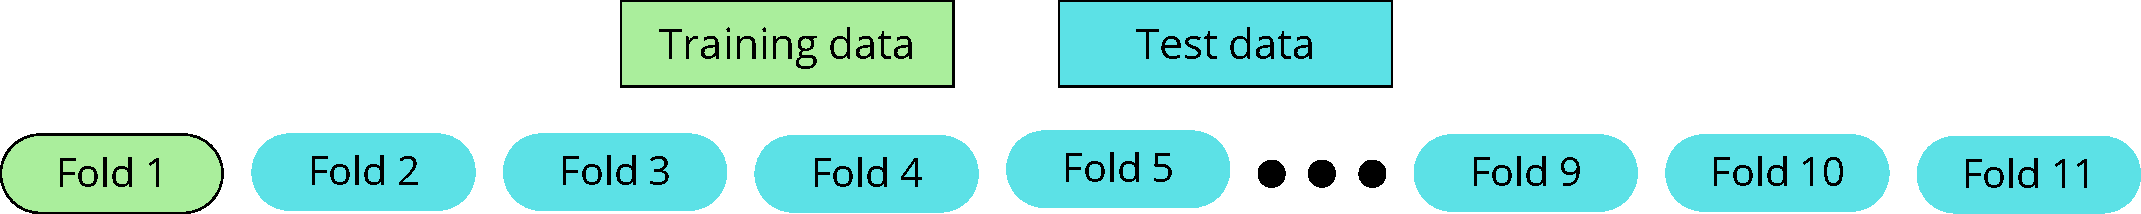
\includegraphics[width=0.9\textwidth]{images/Folds predictions.pdf}
    \caption{Acumulación de predicciones en \textit{key-fold cross-validation}}
    \label{fig:fold-predictions}
\end{figure}

Como vemos en la Figura \ref{fig:fold-predictions}, hemos ido acumulando las predicciones hechas
en cada uno de los \textit{folds} de \textit{test}, para luego calcular las métricas en función
de ellas. Podemos observar, además, que el primer \textit{fold} no se usa para \textit{test},
usándose únicamente para entrenamiento. Sucede algo similar con el último \textit{fold}, que no
es usado para entrenamiento y se usa únicamente para \textit{test}.\\

 

\subsection{Resultados}
